\documentclass[12pt,a4paper]{article}
\usepackage[top=2cm,left=1cm,right=1cm,bottom=2cm]{geometry}
\usepackage{tikz}
 \usepackage[tikz]{bclogo}%
 \usetikzlibrary{calc,intersections}
\usetikzlibrary{arrows.meta}
\usetikzlibrary{decorations.pathmorphing}
\usepackage{amssymb,mathtools,amsthm}
\usepackage{fourier}
\usepackage{tkz-tab}
\usepackage{xcolor}
\usepackage{multicol, array, fancyhdr}
\usepackage{tasks}
\newcommand{\Lim}{\displaystyle\lim}
\renewcommand{\columnseprule}{1pt}
\renewcommand{\arraystretch}{1.5}
% \renewcommand{\displaystyle\frac}[2]{\displaystyle\displaystyle\frac{#1}{#2}}


%======================================================
\newtheoremstyle{mystyle}
  {\topsep}% espace avant
  {\topsep}% espace après
  {\upshape}% police du corps du théorème
  {}% indentation (vide pour rien, \parindent)
  {\bfseries\sffamily}% police du titre du théorème
  { :\newline}% ponctuation après le théorème
  { }% après le titre du théorème (espace ou \newline)
  {%
    \rule[0.5\baselineskip]{0.5\textwidth}{1pt}%
    \newline\fcolorbox{black}{white}{%
      \thmname{#1}\thmnumber{ \textup{#2}}\thmnote{ \textnormal{(#3)}}%
    }%
    
    % \vspace{0.5em} % Adjust vertical space after the title
  }% spécifications du titre

\theoremstyle{mystyle}
\newtheorem{exo}{Exercice}

%======================================================



\begin{document}


\pagestyle{fancy}
\fancyhf{} % clear all header and footer fields
\fancyhead[L]{Lycée : Zitoun \hspace{1.5cm} Année scolaire : 2024-2025} % Left header
\fancyhead[C]{ \hspace{4cm} Niveau : 2BAC PC} % Right-Center header
\fancyhead[R]{Prof. Othmane Laksoumi} % Right header
\fancyfoot[C]{\thepage} % Footer


\begin{center}
    \textbf{\Large Limites et continuité}
\end{center}
\begin{multicols*}{2}



\begin{exo}
Étudier la continuité de la fonction $f$ en $x_0$:

\begin{enumerate}
    \item
    \[
    \begin{cases} 
        f(x) =\displaystyle\frac{x^3 - 1}{x^2 - 3x + 2} & \text{si } x \neq 1, \\
        f(1) = -3 
    \end{cases}
    \quad x_0 = 1
    \]

    \item
    \[
    \begin{cases} 
        f(x) =\displaystyle\frac{x^2 - 2x - 3}{x^2 - 7x + 12} & \text{si } x \neq 3, \\
        f(3) =-4
    \end{cases}
    \quad x_0 = 3
    \]

    \item
    \[
    \begin{cases} 
        f(x) =\displaystyle\frac{\sqrt{1 + x^2} - 1}{2x} & \text{si } x \neq 0, \\
        f(0) =1
    \end{cases}
    \quad x_0 = 0
    \]

    \item
    \[
    \begin{cases} 
        f(x) =\displaystyle\frac{x^2 + 5x + 6}{x^2 + 8x + 12} & \text{si } x > -2, \\
        f(x) =\displaystyle\frac{\sqrt{x + 6} - 2}{x + 2} & \text{si } x < -2, \\
        f(-2) =\displaystyle\frac{1}{4} & \text{si } x = -2,
    \end{cases}
    \quad x_0 = -2
    \]

    \item
    \[
    \begin{cases} 
        f(x) =\displaystyle\frac{|x^2 - 3x + 2|}{x^2 - 4} & \text{si } x \neq 2, \\
        f(2) =\displaystyle\frac{1}{4}
    \end{cases}
    \quad x_0 = 2
    \]

    \item
    \[
    \begin{cases} 
       f(x) = 1 + \displaystyle\frac{1}{|x - 2|} & \text{si } x \neq 2, \\
       f(2) = 1
    \end{cases}
    \quad x_0 = 2
    \]
\end{enumerate}
\end{exo}

\begin{exo}
     Dans chacun des cas suivants, déterminer la
valeur du réel $a$ pour que la fonction $f$ soit continue en $x_0$ :
\begin{enumerate}
    \item 
    \[
    \begin{cases} 
        f(x) =\displaystyle\frac{\sqrt{x - 1}}{x^2 - 3x + 2} & \text{si } x \neq 1, \\
        f(1) =a
    \end{cases}
    \quad x_0 = 1
    \]

    \item 
    \[
    \begin{cases} 
        f(x) =\displaystyle\frac{\sin(\pi x)}{x - 1} & \text{si } x \neq 1, \\
        f(1) =a
    \end{cases}
    \quad x_0 = 1
    \]

    \item 
    \[
    \begin{cases} 
        f(x) =\displaystyle\frac{\tan(x) - \sqrt{3}}{x - \displaystyle\frac{\pi}{3}} & \text{si } x \neq \displaystyle\frac{\pi}{3}, \\
        f\left(\displaystyle\frac{\pi}{3}\right) =a
    \end{cases}
    \quad x_0 = \displaystyle\frac{\pi}{3}
    \]

    \item 
    \[
    \begin{cases} 
        f(x) =\displaystyle\frac{a x^2 + (a + 1)x + 1}{2x^2 + x - 1} & \text{si } x \neq -1, \\
        f(-1) =\displaystyle\frac{1}{3}
    \end{cases}
    \quad x_0 = -1
    \]
\end{enumerate}

\end{exo}

\begin{exo}
    Dans chacun des cas suivants, montrer que la fonction $f$ est continue sur son ensemble de définition.
    \begin{enumerate}
        \item $f(x) = x^2 + 3x + \cos{x}$
        \item $f(x) = \sqrt{x^2 - 5x - 6}$
        \item $f(x) = \displaystyle\frac{3x^2 + 5x - 4}{x^2 + 3} \sqrt{2x^2 - x + 3}$
        \item $f(x) = \displaystyle\frac{\sin{x}}{x^2 -3x +2}$
        \item $f(x) = \cos(-3x^2 + 5)$
    \end{enumerate}
\end{exo}

\begin{exo}
    Soit $f$ la fonction numérique définie sur $\mathbb{R}$ par :
    $$
    \begin{cases}
        f(x) = |x| + x + 1 &\text{si } x \leq 1\\
        f(x) = \sqrt{x}(x^2+2) & \text{si } x > 1
    \end{cases}
    $$
    \begin{enumerate}
        \item Montrer que la fonction $f$ est continue sur chacun des intervalles $]-\infty; 1[$ et $]1;+\infty[$.
        \item Montrer que $f$ est continue en $1$. Que déduit-on?
    \end{enumerate}
\end{exo}

\begin{exo}
    Soit $f$ la fonction numérique définie sur $\mathbb{R}-{1}$ par :
    $$f(x) = \frac{2x}{x-1}$$
    \begin{enumerate}
        \item Dresser le tableau de varoations de $f$.
        \item Déterminer l'image de chacun des intervalles suivants par ma fonction $f$ : 
        
        $I = ]1;3]\quad;\quad J = ]1;+\infty[\quad;\quad K = \mathbb{R}^-$
        
        $L = ]-\infty ; 1[$
    \end{enumerate}
\end{exo}

% =======================================================================

\begin{exo}
    Dans chacun des cas suivants, montrer que l'équation proposée admet au moins une solution dans $I$ :
    \begin{enumerate}
        \item $x^3 - 2x^2 - 1 = 0\quad\quad;\quad I = [2;3]$
        \item $x^4 - 2x - \sqrt{x} + 1 = 0\quad\quad;\quad I = ]0;1[$
        \item $x - 2\sin{x} = 0\quad\quad;\quad I = \left]\displaystyle\frac{\pi}{3};\pi\right[$
        \item $\displaystyle\frac{3}{2}x - \tan{x} = 0\quad\quad;\quad I = \left]\displaystyle\frac{\pi}{4};\displaystyle\frac{\pi}{3}\right[$
    \end{enumerate}
\end{exo}

\begin{exo}
    Dans chacun des cas suivants, montrer que l'équation proposée admet une solution unique dans $I$ :
    \begin{enumerate}
        \item $2x^3 + 3x - 3 = 0 \quad\quad;\quad I = [0;1]$
        \item $x^4 + 2x - 3 = 0\quad\quad;\quad I = \left[\displaystyle\frac{1}{2};\sqrt{2}\right]$
        \item $\tan{x} = x + 1\quad\quad;\quad I = \left[0;\displaystyle\frac{\pi}{2}\right]$
    \end{enumerate}
\end{exo}

\begin{exo}
    Soit $f$ la fonction numérique définie sur $\mathbb{R}$ par :
    $$f(x) = 4x^3-3x-\frac{1}{2}$$
    \begin{enumerate}
        \item Calculer : $f(-1)\quad;\quad f\left(-\displaystyle\frac{1}{2}\right)\quad;\quad f(0)\quad;\quad f(1)$
        \item En déduire que l'équation $f(x) = 0$ admet au moins trois solutions dans l'intervalle $[-1;1]$.
    \end{enumerate}
\end{exo}
    
\begin{exo}
      Soit $f$ une fontion continue sur les deux intervalles $]-\infty; 2[$ et $]2;+\infty[$ et dont le tableau de variations est donné par :
      
        \hspace{-10mm}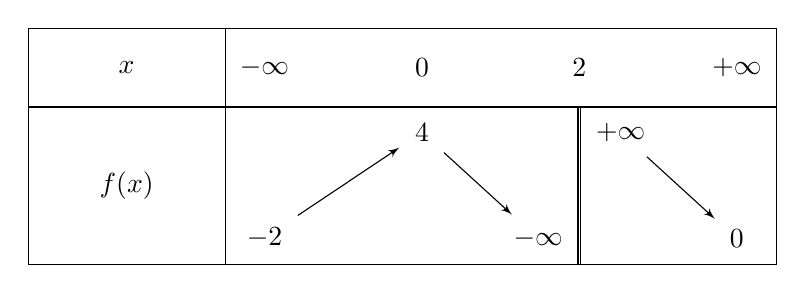
\begin{tikzpicture}
          \tkzTabInit[lgt=2.5, espcl=2] {$x$/1, $f(x)$/2}{$-\infty$, $0$, $2$, $+\infty$}
          \tkzTabVar{-/$-2$, +/4, -D+/ $-\infty$/$+\infty$, -/0}
        \end{tikzpicture}
        \begin{enumerate}
            \item Déterminer : 
            
            $f(]-\infty; 0])\quad;\quad f([0;2[)\quad;\quad f(]2;+\infty[)\\ f(]-\infty ; 2[)$
            \item Déterminer le nombre de solutions de l'équation $f(x) = 0$.
            \item Même question pour les équations :
            $$f(x) = 3\quad;\quad f(x)=-2\quad;\quad f(x) = 7$$
        \end{enumerate}
\end{exo} 

\begin{exo}
    Soit $f$ la fonction définie par : $f(x) = x^3 - 3x +1$.
    \begin{enumerate}
        \item Montrer que l'équation $f(x) = 0$ admet une solution unique $\alpha$ dans l'intervalle $]-1;1[$.
        \item Déterminer un encadrement de $\alpha$ d'amplitude $0,25$.
    \end{enumerate}
\end{exo}

\begin{exo}
    Soit $f$ la fonction numérique définie sur l'intervalle $\left[\displaystyle\frac{1}{4};+\infty\right[$ par : $f(x) = 2x^2 - x + 1$.
    \begin{enumerate}
        \item Montrer que la fonction $f$ admet une fonction réciproque $f^{-1}$ définie sur un intervalle $J$ à déterminer.
        \item Dresser le tableau de variations de la fonction $f^{-1}$.
        \item Déterminer $f^{-1}(x)$ pour tout $x\in J$.
    \end{enumerate}
\end{exo}

\begin{exo}
Dans chacun des cas suivants, montrer que $f$ définie sur l'intervalle $I$ admet une fonction réciproque définie sur un intervalle $J$ à déterminer, puis donner une expression de $f^{-1}(x)$ :

\begin{enumerate}
    \item $f(x) = \displaystyle\frac{x^2}{x - 2}$ ; \quad $I = [5; +\infty[$
    \item $f(x) = -2(x - 1)^2 + 5$ ; \quad $I = [1; +\infty[$
    \item $f(x) = x^2 - 6x + 5$ ; \quad $I = ]-\infty ; 3]$
    \item $f(x) = \displaystyle\frac{x}{\sqrt{x^2 + 1}}$ ; \quad $I = \mathbb{R}^+$
    \item $f(x) = \left( \sqrt{3 - x }+ 1 \right)^2$ ; \quad $I = ]-\infty ; 3]$
    \item $f(x) = -\sqrt{x^2 - 2}$ ; \quad $I = [1; +\infty[$
    \item $f(x) = 2x - \sqrt{x}$ ; \quad $I = \left[ 0 ; \frac{1}{16} \right]$
\end{enumerate}

\end{exo}

% ======================================================================

\begin{exo}
\text{ }
    \begin{enumerate}
    \item Simplifier les nombres suivants :
    \[
    a = \frac{\sqrt{18} \times \sqrt{\sqrt[3]{256}} \times \sqrt[4]{64}}{\sqrt[3]{1024} \times \sqrt[6]{64\times 10^6}}, \quad
    b = \frac{\sqrt[15]{3} \times \sqrt[3]{9} \times (\sqrt{9})^3}{\sqrt[4]{27} \times \sqrt{\sqrt{3}}}
    \]
    \[
    c = \frac{\sqrt[4]{2048} \times \sqrt[4]{160000}}{\sqrt[8]{4096} \times \sqrt[3]{\sqrt{256}} \times \sqrt{512}}
    \]

    \item Simplifier les nombres suivants :
    \[
    x = \left(27\right)^{\frac{2}{3}} \times \left(16\right)^{\frac{3}{4}} - \frac{2}{\sqrt[3]{8^{-2}}} + \frac{\sqrt[5]{2}}{4^{-\frac{2}{5}}}
    \]
    \[
    y = \frac{(81)^{\frac{2}{9}} \times \left(27\right)^{\frac{1}{4}} \times 9^{\frac{5}{2}}}{3^{\frac{14}{3}}}
    \]
    \[
    z = \frac{a^{\frac{5}{3}} \times \left(\sqrt[4]{\frac{1}{a^2}}\right)^3 \times b^{\frac{5}{2}}}{\left(a^{\frac{5}{3}}\right)^{\frac{2}{3}} \times \sqrt[5]{b^{-\frac{3}{4}}}}
    \]
    (ici \(a, b \in \mathbb{R}^*_{+}\)).

    \item Comparer les deux nombres : \(\sqrt[5]{91}\) et \(\sqrt[3]{15}\)

    \item Ordonner dans l’ordre croissant les nombres : 
    \[
    A = \sqrt{2}, \quad B = \sqrt[3]{4}, \quad C = \sqrt[6]{5}, \quad D = \sqrt[4]{3}
    \]

    \item Écrire les dénominateurs des nombres suivants sous la forme d’un nombre rationnel :
    \[
    \frac{1}{2 \sqrt[3]{4}}, \quad \frac{2}{\sqrt[3]{3} - 1}, \quad \frac{\sqrt[4]{5} + \sqrt[4]{2}}{\sqrt[4]{5} - \sqrt[4]{2}}, \quad \frac{1}{1 + \sqrt[3]{2} + \sqrt[3]{4}}
    \]
\end{enumerate}
\end{exo}

\begin{exo}
    Résoudre dans $\mathbb{R}$ les équations et les inéquations suivantes :
    \begin{multicols}{2}
        \begin{enumerate}
            \item $x^8 - 9 = 0$
            \item $8x^3 + 27 = 0$
            \item $x^7 = \sqrt{2}$
            \item $\sqrt[3]{x} = \sqrt[6]{7}$
            \item $\sqrt[3]{1 + x} + \sqrt[3]{1 - x} = 2$
            \item $\sqrt{x} + \sqrt[3]{x} = 12$
            \item $4x^3 - 125 \geq 0$
            \item $\sqrt{2x+1} < 3 + \sqrt{x + 2}$
            \item $\sqrt{x - 1} - \sqrt[3]{x - 2} > 1$
        \end{enumerate}
    \end{multicols}
\end{exo}

\begin{exo}
Calculer les limites suivantes :
    \[
\lim_{x \to +\infty} \frac{x}{\sqrt[3]{x} - 1} ; \quad
\lim_{x \to -\infty} \frac{\sqrt[3]{x - x^3}}{2 - x} ; \quad
\lim_{x \to 0} \frac{\sqrt[3]{1 - x} - 1}{\sin x}
\]

\[
\lim_{x \to 2} \frac{x - \sqrt[3]{x + 6}}{3 - \sqrt{2x + 5}} ; \quad
\lim_{x \to 1} \frac{\sqrt[3]{x + 7} - 2}{\sqrt[4]{x} - 1} ; \quad
\lim_{x \to 4} \frac{\sqrt[3]{5 - x} - 1}{2 - \sqrt[3]{x + 4}}
\]

\[
\lim_{x \to +\infty} x - \sqrt[3]{x} - \sqrt{x} ; \quad
\lim_{x \to 2} \frac{\sqrt[3]{x + 6} - \sqrt{x + 2}}{x - 2}
\]

\[
\lim_{x \to +\infty} \frac{\sqrt{x} - \sqrt[3]{x}}{\sqrt{x} + \sqrt[6]{x}}
\]
\end{exo}



\end{multicols*}



\end{document}